\newcommand{\tabin}[1]{\begin{center}{\footnotesize\setlength{\tabcolsep}{3pt}\input{#1}}\end{center}}

\section{Robustness study in detail}\label{app:rob}
\textbf{Setup.} The 100 generated bills of \texttt{examples/final\_run} (made after training with seeds no earlier step used) were degraded after rendering, in ten conditions, and read by the fine-tuned model with per-field confidences. Blur is a Gaussian blur of the given radius; tilt rotates the page by the given angle on a grey background; fading blends the print towards white until the given share of its contrast is left. ``Highlighted'' is the share of fields whose confidence is below the calibrated threshold (0.9884); ``errors caught'' is the share of wrong fields that are highlighted; ``unflagged right'' is the share of correct fields among those not highlighted; ``missed-error bills'' are bills holding a wrong field that is not highlighted; ``retake prompt'' is the share of bills for which the app's photo-quality check would ask for a new photo. These are degraded renders of generated bills and say nothing certain about real photographs.

\tabin{data/app_deg_acc.tex}
\tabin{data/app_deg_conf.tex}

\textbf{Reading the tables.} Blur and fading hardly change the reading until blur is heavy; at 3 px the field F1 is 0.943 and only 84\% of grand totals are right, but 96\% of the wrong fields are highlighted. At 5 px reading fails (F1 0.082) and 97\% of fields are highlighted, so the screen tells the user there is little to trust. Tilt is harder for the model and for its confidence: at 15 degrees one bill in three holds a wrong field that is not highlighted. The retake prompt is over-cautious on these bills (13\% on clean ones, 95\% at 1.5 px of blur, 100\% when the print is faded to a quarter of its contrast although the model still reads those bills at F1 0.984) and does not react to tilt. It is a prompt only (``Use it anyway'' continues), and its thresholds come from CORD and SROIE photos; we did not retune them on generated bills.

\subsection*{Straightening tilted photos}
Because tilt hurt most, we tested a deskew filter (the page angle is estimated from the text lines and undone) on the same bills tilted by 0, 4, 8 and 15 degrees. The estimator searches up to 10 degrees, so the 15-degree bills are corrected only partly. It helps clearly from 8 degrees up and costs 0.3 points of field F1 on untilted bills, so the app applies it only to photos tilted by 6 degrees or more (setting \texttt{AUTO\_DESKEW\_DEG}); the angle estimate takes about 30 ms per photo.

\tabin{data/app_deskew.tex}
\def\deskewlabels{0$^\circ$,4$^\circ$,8$^\circ$,15$^\circ$}

\begin{figure}[!ht]
\centering
\begin{tikzpicture}
\begin{axis}[ybar,width=0.62\textwidth,height=4.2cm,bar width=11pt,xtick=data,xticklabels/.expanded={\deskewlabels},xlabel={tilt of the bill},ylabel={field F1},ymin=0.88,ymax=1.0,ymajorgrids,legend style={at={(0.5,1.03)},anchor=south,legend columns=2},enlarge x limits=0.2]
\addplot[fill=ash,draw=ink] table[x=x,y=y]{data/app_deskew_asis.dat};
\addplot[fill=brick,draw=ink] table[x=x,y=y]{data/app_deskew_fix.dat};
\legend{read as is,straightened first}
\end{axis}
\end{tikzpicture}
\caption{Field F1 on 100 tilted generated bills, with and without straightening.}
\end{figure}

\section{Mistakes on clean bills}\label{app:err}
On the 100 unseen generated bills read without any degradation, 21 bills contain at least one wrong field and there are 27 wrong fields in all (Table~\ref{tab:errs}). Twenty-six are a misread unit price whose line total is right; one is a wrong charge type. A unit price is redundant (quantity times price must equal the line total), which is why the correction screen can catch it and why the one-tap suggestion of Table~\ref{tab:repair} works: it proposes the line total divided by the quantity, and on these bills it fixed all 26 wrong prices and changed no correct one. The suggestion is only offered when the division gives a whole number of paise, it is never applied silently, and it has only been measured on generated bills.

\begin{table}[!ht]\centering\footnotesize
\begin{tabular}{@{}lrlr@{}}
\toprule
Kind of mistake & Count & Kind of mistake & Count \\
\midrule
Item name misread & 0 & Charge type wrong & 1 \\
Quantity misread & 0 & Charge amount wrong & 0 \\
Unit price misread & 26 & Charge missed & 0 \\
Line total misread & 0 & Charge added & 0 \\
Item missed & 0 & Subtotal wrong & 0 \\
Item added & 0 & Grand total wrong & 0 \\
\bottomrule
\end{tabular}

\caption{Wrong fields by kind, 100 unseen generated bills.}\label{tab:errs}
\end{table}
\begin{table}[!ht]\centering\footnotesize
\begin{tabular}{@{}lrr@{}}
\toprule
Rate suggestion on the same 100 bills & Before & After \\
\midrule
Field F1 & 0.9879 & 0.9969 \\
Bills with every rate right & 80 of 100 & 100 of 100 \\
Suggestions made & \multicolumn{2}{r}{26} \\
Suggestions that fix a wrong rate & \multicolumn{2}{r}{26} \\
Correct rates broken & \multicolumn{2}{r}{0} \\
\bottomrule
\end{tabular}

\caption{The one-tap rate suggestion, measured on the same bills.}\label{tab:repair}
\end{table}

\textbf{Examples.} Table~\ref{tab:exs} lists the first misreads from the bills we saved. The error analysis kept the details of 12 bills; in those, 15 of the 15 misread unit prices were among the fields the app highlights for review, so the user is pointed at the mistake before splitting.

\begin{table}[!ht]\centering\footnotesize
\begin{tabular}{@{}llllrl@{}}
\toprule
Bill & Item & Field & Read & Label & Highlighted \\
\midrule
final\_001 & Mutton Curry & unit price & 310 & 305 & yes \\
final\_018 & Samosa & unit price & 60 & 30 & yes \\
final\_020 & Mutton Curry & unit price & 280 & 290 & yes \\
final\_020 & Cold Coffee & unit price & 165.5 & 160.5 & yes \\
final\_023 & Cold Coffee & unit price & 115 & 90 & yes \\
final\_027 & Veg Sandwich & unit price & 115 & 80 & yes \\
final\_028 & Mutton Curry & unit price & 260 & 255 & yes \\
final\_034 & Veg Sandwich & unit price & 77.5 & 55.5 & yes \\
final\_040 & Veg Thali & unit price & 125 & 125.5 & yes \\
\bottomrule
\end{tabular}

\caption{Misread unit prices (first nine of the saved examples).}\label{tab:exs}
\end{table}

\section{Real receipt scans: where the main task fails}\label{app:sroie}
SROIE labels give only the shop, date, address and total, so the main task (items and charges) was trained on CORD and generated bills but never on SROIE-style images. We ran the fine-tuned model on 8 real SROIE scans kept locally (4 test, 4 training scans). With the main task it returned no items on any of them (Table~\ref{tab:sroie}); with each of six image enhancements applied first, it still returned none (Table~\ref{tab:sroievar}). The raw text shows why: the model begins the main-task answer and then writes the four SROIE fields, with a mismatched closing tag, instead of items:

\begin{center}\begin{minipage}{0.95\textwidth}\scriptsize\begin{verbatim}
<s_splitsnap><s_items><s_name> OJOC MARKETING SDN BHD</s_company>
<s_date> 15/01/2019</s_date>
<s_address> NO 2 & 4, JALAN BAYU 4, BANDAR SERI ALAM, 81750 MASAI, JOHOR</s_address>
<s_total> 193</s_total></s>
\end{verbatim}\end{minipage}\end{center}
(main-task output for the first scan, read from \texttt{generate\_raw} in \texttt{splitsnap/infer.py}; not saved to a results file). The auxiliary SROIE task reads the same scans well (last four columns of Table~\ref{tab:sroie}: date 8 of 8, company 7, total 7, address 4 exact). The app uses that reading as a fallback: when the main task finds no items it shows the shop name and total and offers to enter the items by hand with the total filled in. A fix that reads the items needs the main task trained on real receipt-style images.

\begin{table}[!ht]\centering\footnotesize\setlength{\tabcolsep}{4pt}
\begin{tabular}{@{}lrrrrrr@{}}
\toprule
Scan & Label total & Main task items & Company & Date & Address & Total \\
\midrule
test\_X00016469670 & 193 & 0 & yes & yes & no & yes \\
test\_X51005200931 & 436.2 & 0 & yes & yes & yes & yes \\
test\_X51005230605 & 4.9 & 0 & yes & yes & no & no \\
test\_X51005230616 & 38.9 & 0 & yes & yes & yes & yes \\
train\_X51006328913 & 165 & 0 & yes & yes & yes & yes \\
train\_X51006329399 & 12.15 & 0 & no & yes & no & yes \\
train\_X51006332575 & 62 & 0 & yes & yes & yes & yes \\
train\_X51007135247 & 37.45 & 0 & yes & yes & no & yes \\
\bottomrule
\end{tabular}

\caption{Eight real SROIE scans: main-task items and auxiliary-task exact matches.}\label{tab:sroie}
\end{table}
\begin{table}[!ht]\centering\footnotesize
\begin{tabular}{@{}lr@{}}
\toprule
Image enhancement before reading & Scans with items (of 8) \\
\midrule
none (as is) & 0 \\
clahe & 0 \\
shadow & 0 \\
sharpen & 0 \\
denoise & 0 \\
deskew & 0 \\
shadow+clahe & 0 \\
\bottomrule
\end{tabular}

\caption{Scans for which the main task returned any item, by enhancement applied before reading.}\label{tab:sroievar}
\end{table}

\section{Confidence calibration in detail}\label{app:cal}
The confidence of a field is computed from the probabilities of the tokens that wrote it, in three ways (Table~\ref{tab:agg}); the minimum token probability separates wrong from right fields best and is the one used. Raw scores are already well calibrated; isotonic regression, fitted in two folds split by bill, lowers the expected calibration error further. The data are 4,107 predicted fields from 198 validation bills (CORD and generated; 97.4\% of the fields are correct); SROIE fields carry no confidence. Table~\ref{tab:trade} shows what each choice of highlighted share would buy, and Table~\ref{tab:types} the quality by field type.

\begin{table}[!ht]\centering\footnotesize\setlength{\tabcolsep}{3.5pt}
\begin{tabular}{@{}lrrrrrr@{}}
\toprule
Score & AUROC & ECE raw & ECE calibrated & Cut-off & Errors caught & Unflagged right \\
\midrule
first token & 0.871 & 0.015 & 0.005 & 0.9920 & 60.0\% & 98.9\% \\
mean token & 0.882 & 0.018 & 0.006 & 0.9916 & 63.8\% & 99.0\% \\
minimum token (used) & 0.888 & 0.012 & 0.005 & 0.9884 & 67.6\% & 99.1\% \\
\bottomrule
\end{tabular}

\caption{Three ways to score a field. ECE is expected calibration error.}\label{tab:agg}
\end{table}
\begin{table}[!ht]\centering\footnotesize
\begin{tabular}{@{}rrrr@{}}
\toprule
Fields highlighted & Highlight below & Real errors caught & Unflagged correct \\
\midrule
1\% & 0.5466 & 26\% & 98.1\% \\
2\% & 0.7372 & 38\% & 98.4\% \\
5\% & 0.9596 & 59\% & 98.9\% \\
8\% & 0.9884 & 68\% & 99.1\% \\
10\% & 0.9930 & 69\% & 99.1\% \\
15\% & 0.9976 & 74\% & 99.2\% \\
20\% & 0.9991 & 79\% & 99.3\% \\
\bottomrule
\end{tabular}

\caption{Trade-off for the highlighting threshold (minimum-token score).}\label{tab:trade}
\end{table}
\begin{table}[!ht]\centering\footnotesize
\begin{tabular}{@{}lrrr@{}}
\toprule
Field type & Fields & Accuracy & AUROC \\
\midrule
grand total & 197 & 99.5\% & 0.995 \\
amount & 293 & 98.6\% & 0.985 \\
unit price & 781 & 93.7\% & 0.922 \\
subtotal & 198 & 98.0\% & 0.921 \\
name & 782 & 96.2\% & 0.900 \\
type & 292 & 99.0\% & 0.872 \\
total & 782 & 99.2\% & 0.861 \\
qty & 782 & 99.0\% & 0.700 \\
\bottomrule
\end{tabular}

\caption{Confidence quality by field type. Quantity is the field the score can least separate.}\label{tab:types}
\end{table}

\section{The third processed sample bill}\label{app:bill3}
The main text shows two of the three processed sample bills; this is the third. All three, with every intermediate file (photo, extracted JSON, corrections, corrected bill in the problem statement's schema, split and explanation), are in \texttt{examples/processed\_bills/}.

\needspace{8.2cm}\noindent\begin{minipage}[t]{3.1cm}\vspace{0pt}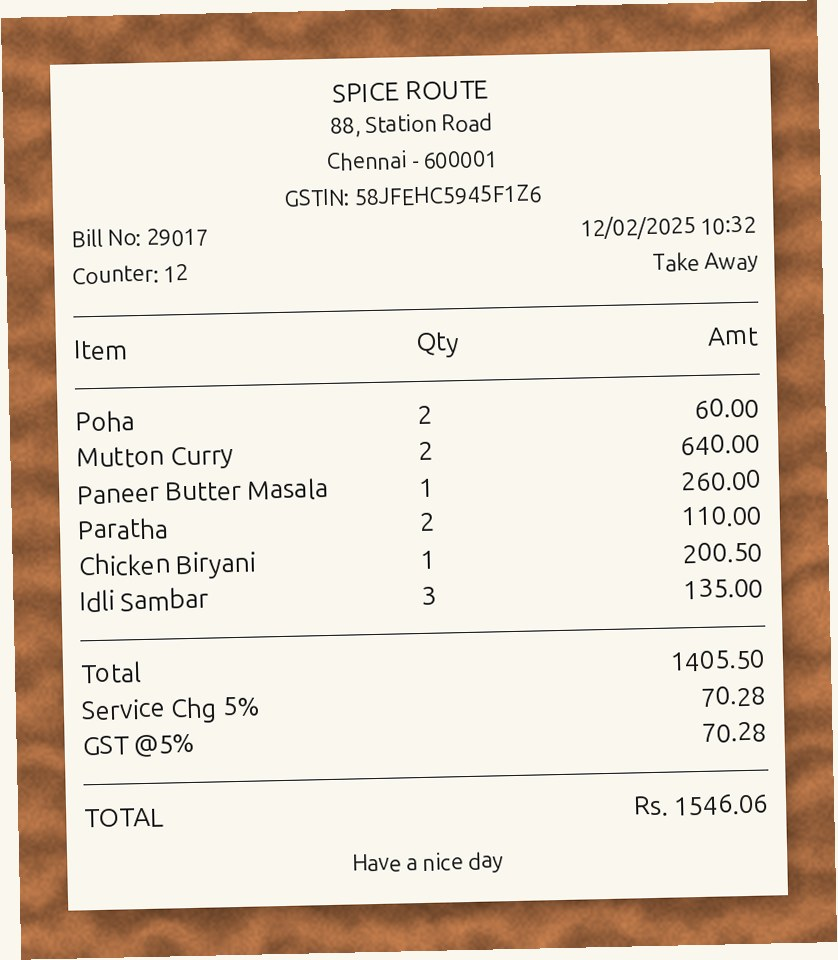
\includegraphics[width=3.1cm]{../examples/final_run/final_017.jpg}\end{minipage}\hfill
\begin{minipage}[t]{\dimexpr\linewidth-3.4cm\relax}\vspace{0pt}{\footnotesize\renewcommand{\arraystretch}{1.0}
\textbf{Bill 3.} The model read 6 items and 2 charges. Corrections made on the check screen: none needed.\\[2pt]
\begin{tabular}{@{}lrrrr@{}}\toprule & Riya & Aman & Sara & Bill\\\midrule
Poha & 20.00 & 20.00 & 20.00 & 60.00 \\
Mutton Curry & 426.67 & 213.33 & 0.00 & 640.00 \\
Paneer Butter Masala & 0.00 & 0.00 & 260.00 & 260.00 \\
Paratha & 110.00 & 0.00 & 0.00 & 110.00 \\
Chicken Biryani & 0.00 & 200.50 & 0.00 & 200.50 \\
Idli Sambar & 0.00 & 67.50 & 67.50 & 135.00 \\
\midrule
Service Charge & 27.83 & 25.07 & 17.38 & 70.28 \\
GST & 27.83 & 25.07 & 17.38 & 70.28 \\
\midrule
Total (Rs) & \textbf{612.33} & \textbf{551.47} & \textbf{382.26} & \textbf{1546.06} \\
\bottomrule\end{tabular}\\[2pt]
\textit{Sara: Poha (1/3 share, Rs 20.00) + Paneer Butter Masala (full, Rs 260.00) + Idli Sambar (1/2 share, Rs 67.50) = Rs 347.50 pre-tax subtotal. Sara's pre-tax subtotal is 24.7\% of the Rs 1405.50 of items on the bill, so Sara carries 24.7\% of each tax, service charge, discount and rounding line. ...}}\end{minipage}
\par\vspace{5pt}


\section{Reproducing every number}\label{app:repro}
{\footnotesize
\begin{tabular}{@{}p{4.6cm}p{6.6cm}p{4.6cm}@{}}
\toprule
Result & Command & Output\\
\midrule
Training, held-out test scores & \texttt{kaggle/run\_kaggle.py} modes \texttt{full}, \texttt{eval} (see README) & \texttt{results/training\_logs/}\\
Before and after fine-tuning & \texttt{scripts/before\_after.py} & \texttt{results/before\_after.json}\\
Degradation study & \texttt{scripts/degradation\_study.py} & \texttt{results/degradation.json}\\
Straightening & \texttt{scripts/deskew\_check.py} & \texttt{results/deskew\_check.json}\\
Error breakdown & \texttt{scripts/error\_analysis.py} & \texttt{results/error\_analysis.json}\\
Rate suggestion & \texttt{scripts/repair\_check.py} & \texttt{results/repair\_check.json}\\
SROIE scans & \texttt{scripts/sroie\_scan\_check.py} & \texttt{results/sroie\_scan\_check.json}\\
Confidence calibration & \texttt{splitsnap/calibrate.py} & \texttt{results/calibration.json}\\
Latency, compile, quantisation & \texttt{scripts/bench\_*.py} & \texttt{results/bench\_*.json}\\
Concurrent load & \texttt{scripts/load\_test.py} & \texttt{results/load\_test.json}\\
Sample bills & \texttt{scripts/make\_sample\_bills.py} & \texttt{examples/processed\_bills/}\\
This report & \texttt{make report} & \texttt{report/SplitSnap\_Model\_Report.pdf}\\
\bottomrule
\end{tabular}}
